 
%---------------------------------------------------------------------------
% Content of Chapter 6 - Implementation
%
%---------------------------------------------------------------------------


\chapter{System deployment and testing}
\label{cha:deployment}

\chabstract{
Although the easiness of use was one of the most notable design goals, a description of deployment, usage, and example sessions is still needed. This chapter focuses solely on these issues. First I will try to cover basic deployment scenarios, from the simplest ones including only a single PC that runs all components - monitored application, Monitoring Hub and GUI up to a distributed approach where all components are spread across multiple hosts. Section~\ref{sec:ch7_working_with} describes roughly the use of the application - installation, starting up and describes in a few steps how to perform the most significant actions within the application. One should treat this section as a minimalistic approach to writing a user guide. The last section of this chapter covers the tests performed on the application. There were two types of tests performed - performance and usability-oriented. With a performance test, I would like to prove that there are no technical caveats when using the application. On the other hand, a usability test describes a real use case of the application, which aims at proving that the application is capable of helping on application performance analysis.

}


%---------------------------------------------------------------------------

%---------------------------------------------------------------------------
% System deployment description.
%
%---------------------------------------------------------------------------


\section{System Deployment}
\label{sec:deployments}

The simplest possible deployment of SemSimMon if depicted in Figure\ref{fig:fib:depl_simple}. As we can see, in this scenario all monitoring components are running on a single machine. User has started monitored application (either single Java app, or even MainSM) either on on his/hers PC or some other remote host (those 2 cases are equal from SemSimMon point of view), then used Monitoring Hub built-in to the Gui component. Transport proxies communicate with monitored applications using localhost or real network interface, and all communication between Monitoring Hub and GUI is done in memory.

\begin{figure}[h]
   \centering
   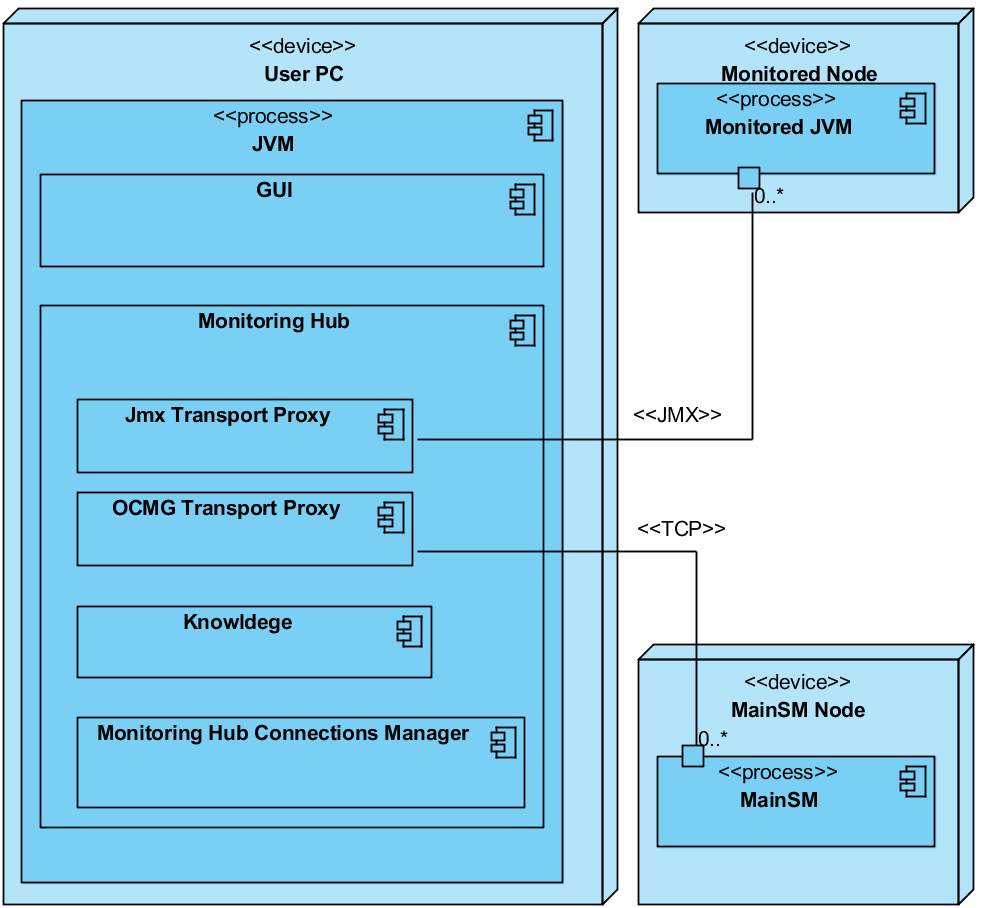
\includegraphics[width=0.6\textwidth]{simplest_deployment}
   \caption{Simplest deployment diagram}
   \label{fib:depl_simple}
 \end{figure}
 
In contrary to previous scenario, Figure~\ref{fig:depl_complex} depicts most complex deployment model. In this case, user has started GUI using own PC, but Monitoring Hub (one or more) runs in separate JVM (either in same, local PC or any other remote host). Connection between those components is established RMI over TCP/IP. Additionally the Monitoring Hub communicates with one or more (again, optionally remote) applications of interest. This deployment is used, when user launches Gui application, monitored applications and chooses to use remote Monitoring Hub while adding resources. This deployment allows most flexible measurements and allows to use system to measure big scale applications.

\begin{figure}[h]
   \centering
   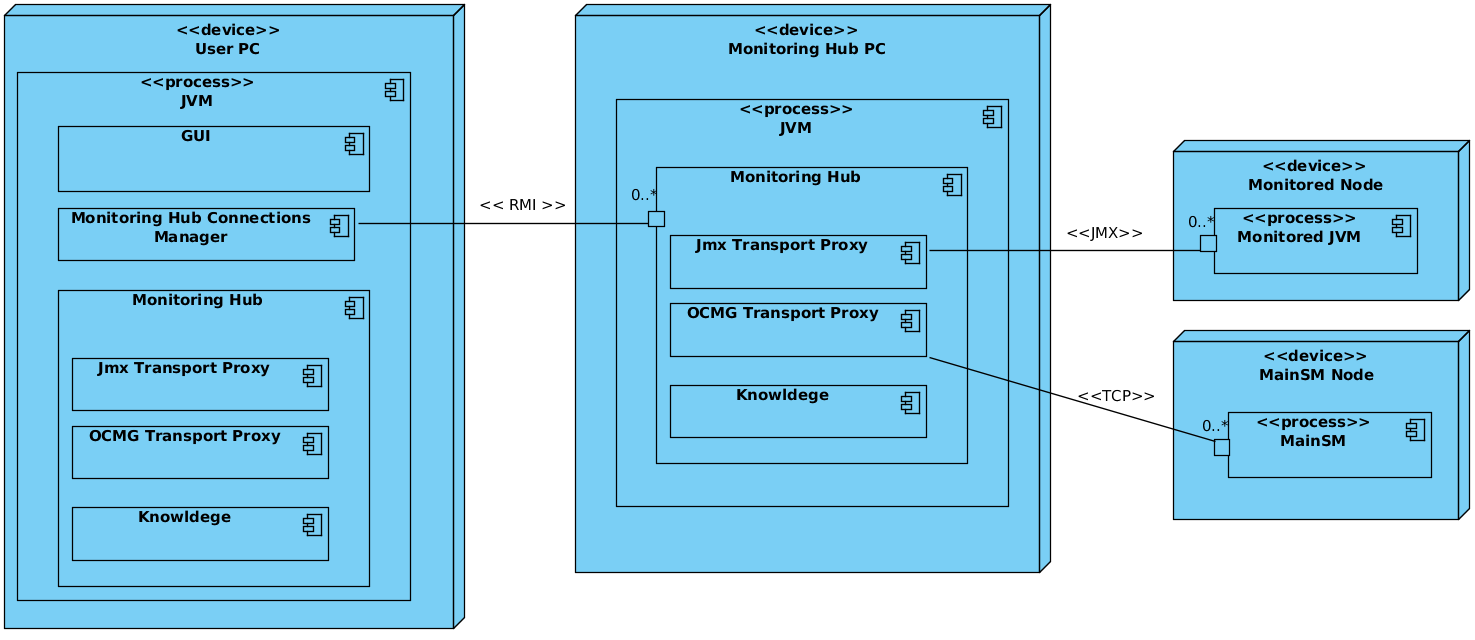
\includegraphics[width=1\textwidth]{distributed_deployment}
   \caption{Distributed deployment diagram}
   \label{fig:depl_complex}
 \end{figure}

%---------------------------------------------------------------------------
% Wokring with semmon.
%
%---------------------------------------------------------------------------


\section{Working with application}
\label{sec:ch7_working_with}

%---------------------------------------------------------------------------
% System tests.
%
%---------------------------------------------------------------------------


\section{Sytem Tests}
\label{sec:ch7_tests}


%---------------------------------------------------------------------------


